\begin{frame}[fragile,t]
  \frametitle{Taylor-mode Automatic Differentiation (Scalar Case)}
  \begin{figure}[t]
    \centering
    \hspace*{-3ex}
    \begin{tikzpicture}
      \matrix (magic)
      [matrix of nodes,
      ampersand replacement=\&,
      nodes={
        anchor=center,
        inner sep=2pt,
      }]
      {
        \only<2->{\textcolor{orange}{\textbf{Taylor}}}
        \&$f^{(0)} = \operatorname{id}$
        \& $f^{(1)} \circ f^{(0)}$
        \& $\dots$
        \& $f^{(L)} \circ \ldots \circ f^{(0)}$
        \\
        \only<1>{%
          \textcolor{blue}{\textbf{Function}}%
          \&%
          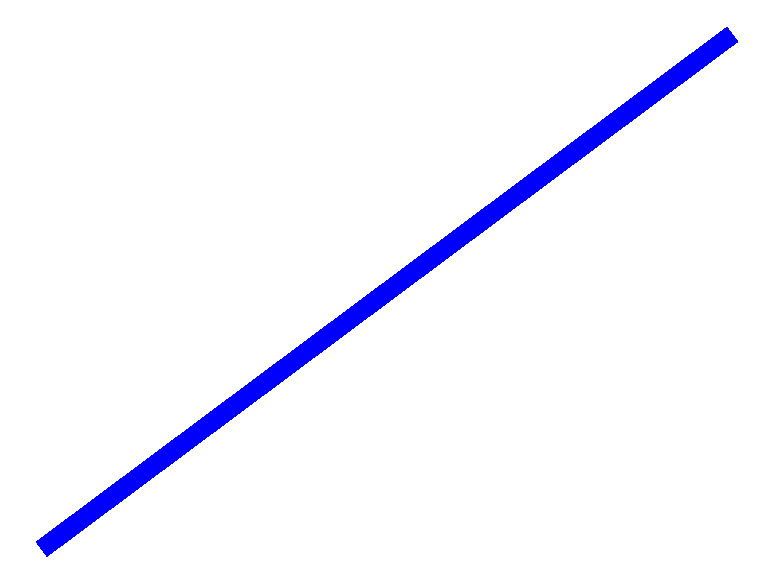
\includegraphics[scale=0.23]{../kfac_pinns_exp/exp48_visualization_taylor_mode/figures/f_0.pdf}%
          \& 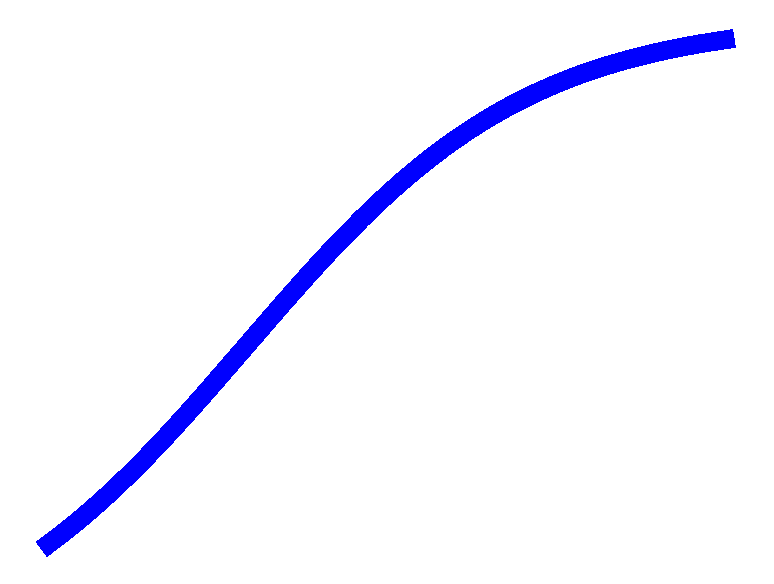
\includegraphics[scale=0.23]{../kfac_pinns_exp/exp48_visualization_taylor_mode/figures/f_1.pdf}%
          \& 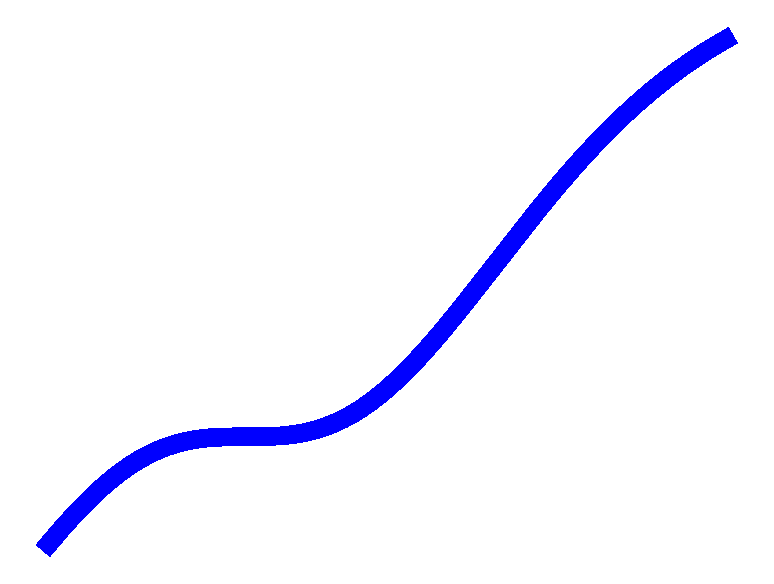
\includegraphics[scale=0.23]{../kfac_pinns_exp/exp48_visualization_taylor_mode/figures/f_2.pdf}%
          \& 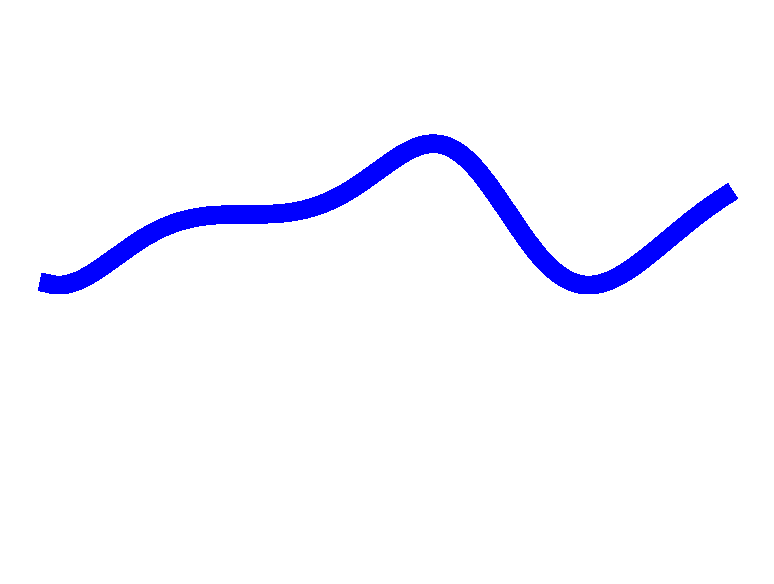
\includegraphics[scale=0.23]{../kfac_pinns_exp/exp48_visualization_taylor_mode/figures/f_3.pdf}%
        }
        \\
        \only<2>{
          \textcolor{orange}{\textbf{0\textsuperscript{th}-order}}
          \& 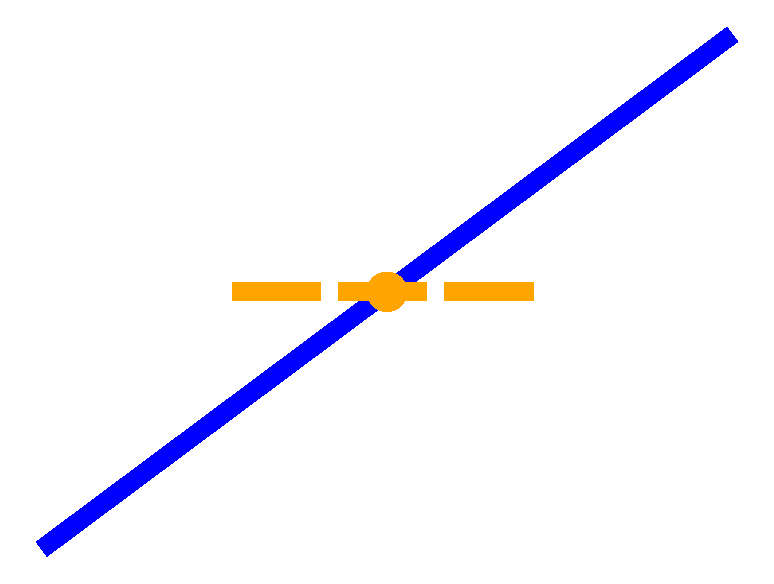
\includegraphics[scale=0.23]{../kfac_pinns_exp/exp48_visualization_taylor_mode/figures/f_0_taylor_0.pdf}
          \& 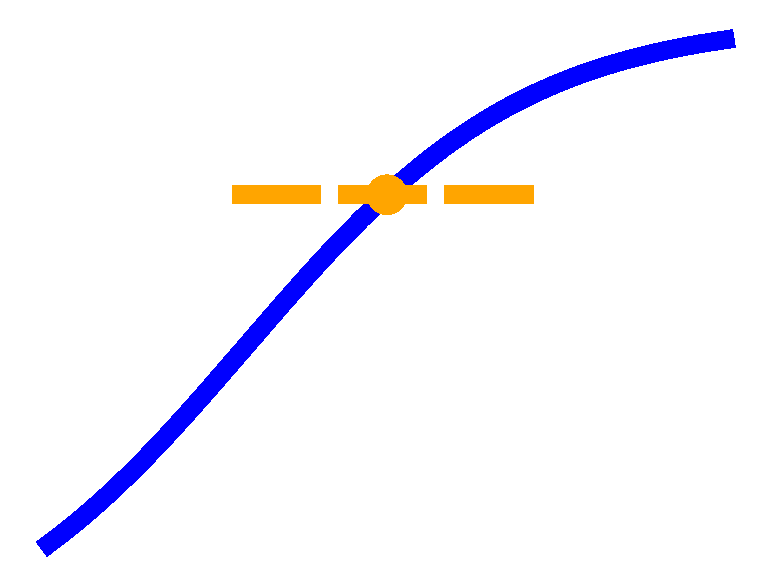
\includegraphics[scale=0.23]{../kfac_pinns_exp/exp48_visualization_taylor_mode/figures/f_1_taylor_0.pdf}
          \& 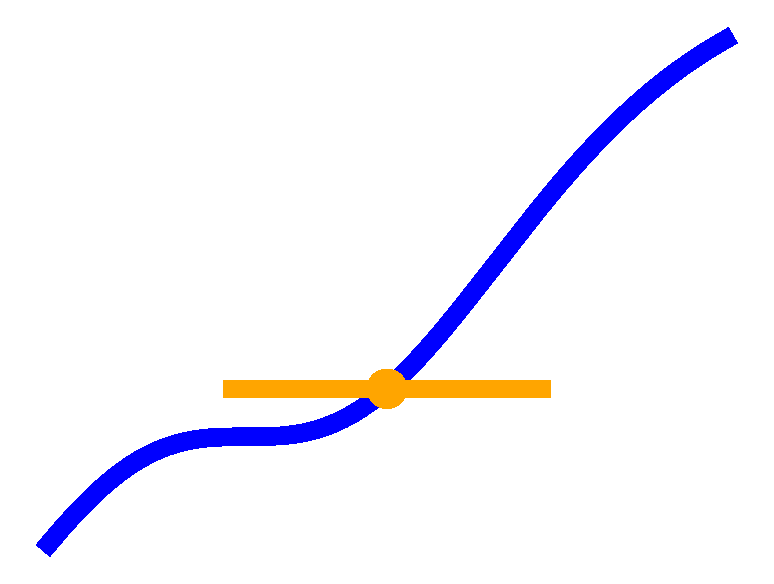
\includegraphics[scale=0.23]{../kfac_pinns_exp/exp48_visualization_taylor_mode/figures/f_2_taylor_0.pdf}
          \& 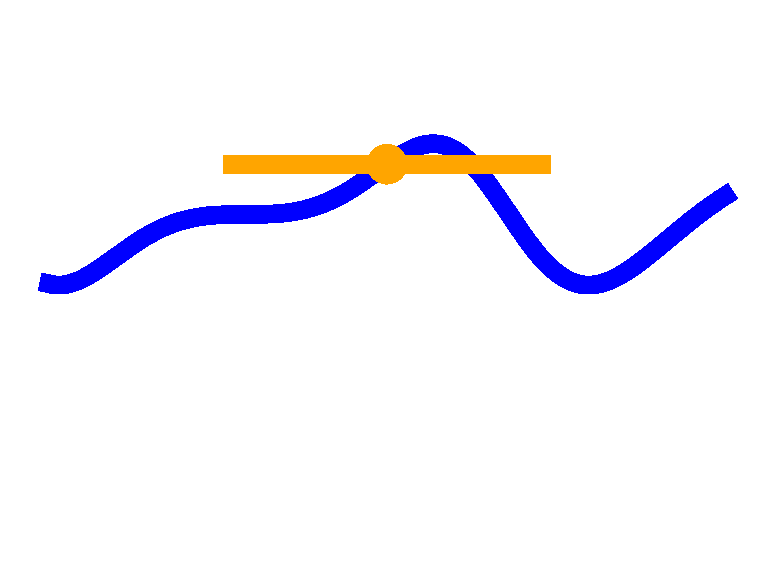
\includegraphics[scale=0.23]{../kfac_pinns_exp/exp48_visualization_taylor_mode/figures/f_3_taylor_0.pdf}
        }
        \only<3>{
          \textcolor{orange}{\textbf{1\textsuperscript{st}-order}}
          \& 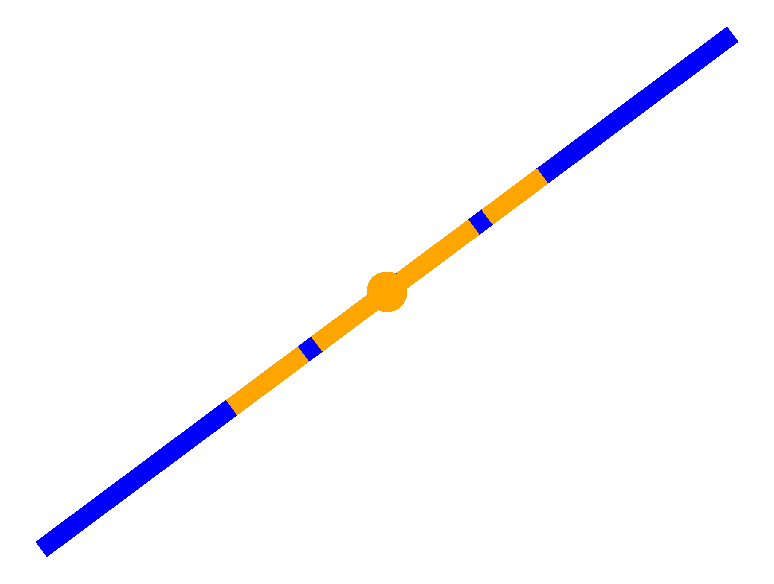
\includegraphics[scale=0.23]{../kfac_pinns_exp/exp48_visualization_taylor_mode/figures/f_0_taylor_1.pdf}
          \& 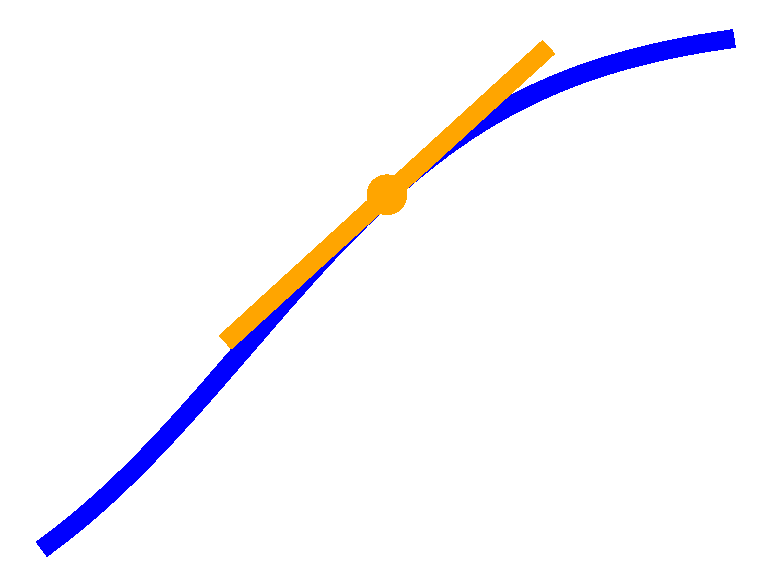
\includegraphics[scale=0.23]{../kfac_pinns_exp/exp48_visualization_taylor_mode/figures/f_1_taylor_1.pdf}
          \& 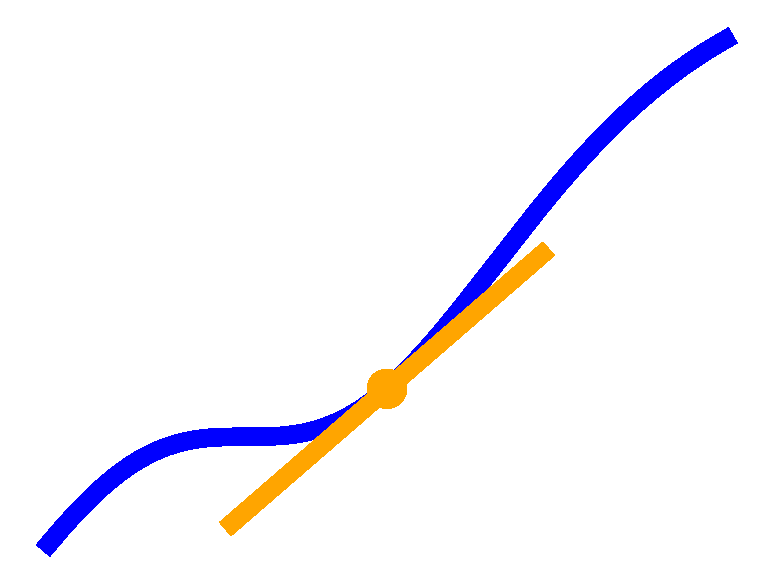
\includegraphics[scale=0.23]{../kfac_pinns_exp/exp48_visualization_taylor_mode/figures/f_2_taylor_1.pdf}
          \& 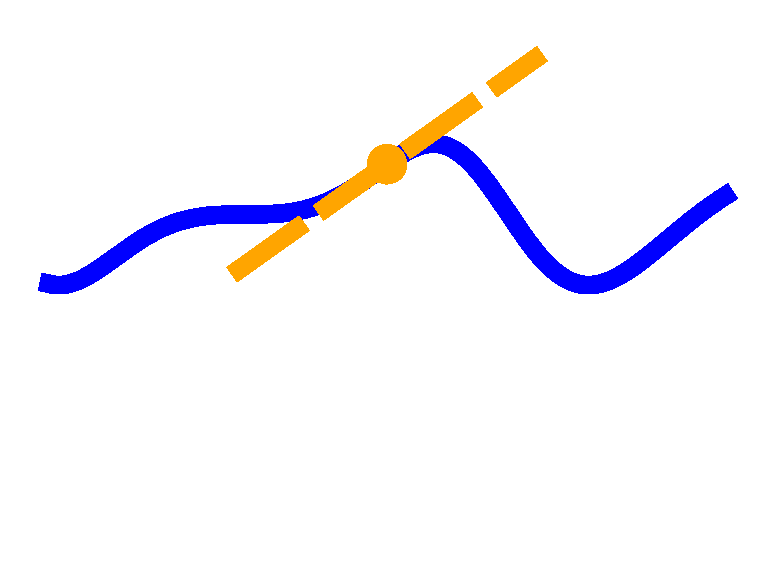
\includegraphics[scale=0.23]{../kfac_pinns_exp/exp48_visualization_taylor_mode/figures/f_3_taylor_1.pdf}
        }
        \only<4>{
          \textcolor{orange}{\textbf{2\textsuperscript{nd}-order}}
          \& 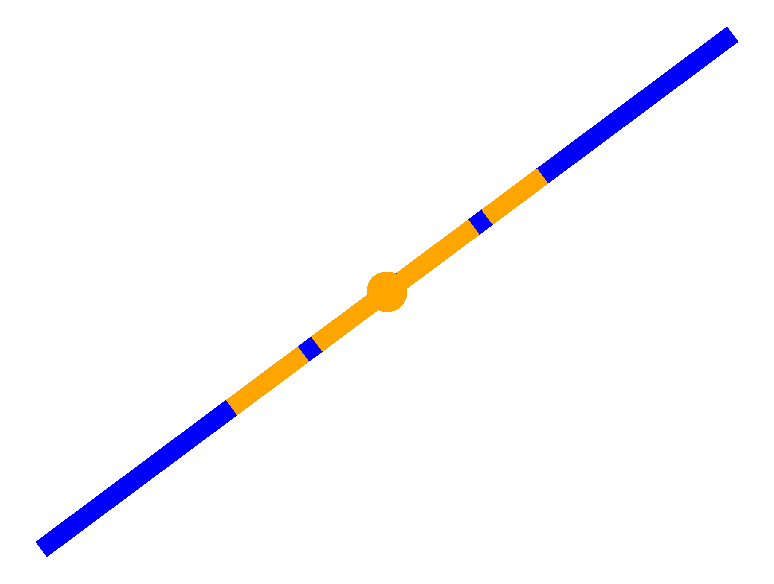
\includegraphics[scale=0.23]{../kfac_pinns_exp/exp48_visualization_taylor_mode/figures/f_0_taylor_2.pdf}
          \& 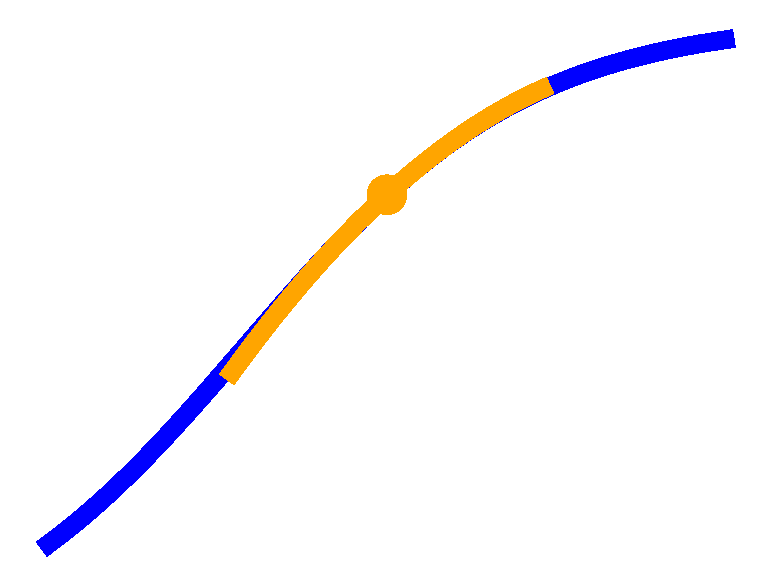
\includegraphics[scale=0.23]{../kfac_pinns_exp/exp48_visualization_taylor_mode/figures/f_1_taylor_2.pdf}
          \& 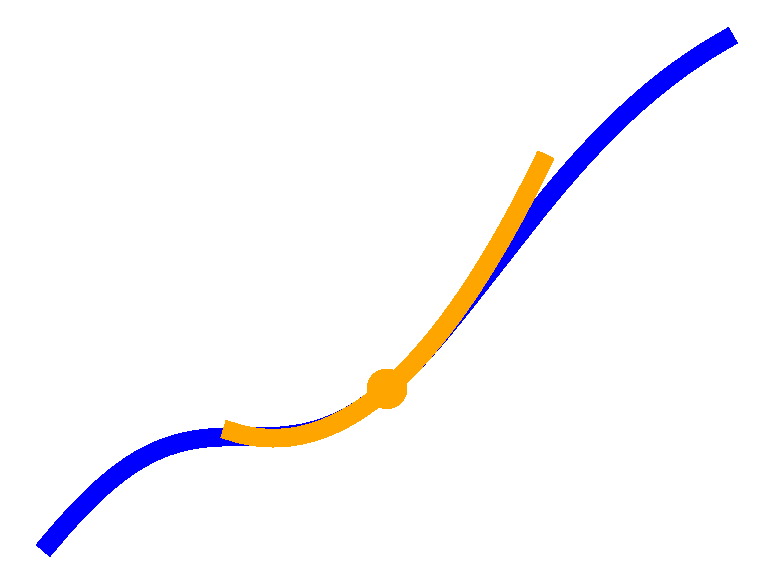
\includegraphics[scale=0.23]{../kfac_pinns_exp/exp48_visualization_taylor_mode/figures/f_2_taylor_2.pdf}
          \& 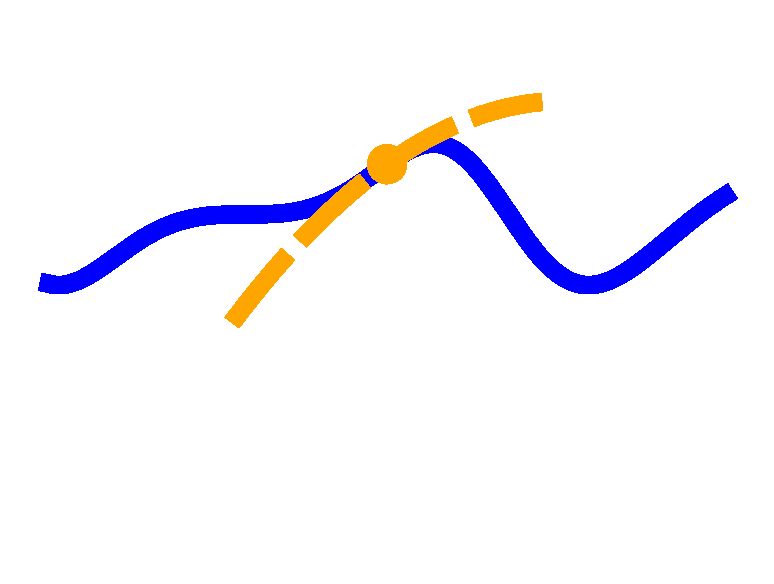
\includegraphics[scale=0.23]{../kfac_pinns_exp/exp48_visualization_taylor_mode/figures/f_3_taylor_2.pdf}
        }
        \\
        \only<2->{
          \& $f^{(0)}(x) = x$
          \& $f^{(1)}(f^{(0)}(x))$
          \&$\dots$
          \&$f^{(L)}(f^{(L-1)}(x))$
        }
        \\
        \only<3->{
          \&$\partial_x f^{(0)}(x) = 1$
          \&$\partial_x f^{(1)}(x)$
          \&$\dots$
          \&$\partial_x f^{(L)}(x)$
        }
        \\
        \only<4->{
          \&$\partial^2_x f^{(0)}(x) = 0$
          \&$\partial^2_x f^{(1)}(x)$
          \&$\dots$
          \&$\partial^2_x f^{(L)}(x)$
        }
        \\
      };
    \end{tikzpicture}
  \end{figure}
\end{frame}
%%% Local Variables:
%%% mode: LaTeX
%%% TeX-master: "../pitch"
%%% End:
